\documentclass[a4paper,10pt,ngerman]{scrartcl}
\usepackage{babel}
\usepackage[T1]{fontenc}
\usepackage[utf8x]{inputenc}
\usepackage[a4paper,margin=2.5cm,footskip=0.5cm]{geometry}

% Die nächsten drei Felder bitte anpassen:
\newcommand{\Aufgabe}{Aufgabe 2: Rechenrätsel} % Aufgabennummer und Aufgabennamen angeben
\newcommand{\TeilnahmeId}{63175}                  % Teilnahme-ID angeben
\newcommand{\Name}{Lars Noack}             % Name des Bearbeiter / der Bearbeiterin dieser Aufgabe angeben


% Kopf- und Fußzeilen
\usepackage{scrlayer-scrpage, lastpage}
\setkomafont{pageheadfoot}{\large\textrm}
\lohead{\Aufgabe}
\rohead{Teilnahme-ID: \TeilnahmeId}
\cfoot*{\thepage{}/\pageref{LastPage}}

% Position des Titels
\usepackage{titling}
\setlength{\droptitle}{-1.0cm}

% Für mathematische Befehle und Symbole
\usepackage{amsmath}
\usepackage{amssymb}

% Für Bilder
\usepackage{graphicx}

% Für Algorithmen
\usepackage{algpseudocode}

% Für Quelltext
\usepackage{listings}
\usepackage{color}
\definecolor{mygreen}{rgb}{0,0.6,0}
\definecolor{mygray}{rgb}{0.5,0.5,0.5}
\definecolor{mymauve}{rgb}{0.58,0,0.82}
\lstset{
  keywordstyle=\color{blue},commentstyle=\color{mygreen},
  stringstyle=\color{mymauve},rulecolor=\color{black},
  basicstyle=\footnotesize\ttfamily,numberstyle=\tiny\color{mygray},
  captionpos=b, % sets the caption-position to bottom
  keepspaces=true, % keeps spaces in text
  numbers=left, numbersep=5pt, showspaces=false,showstringspaces=true,
  showtabs=false, stepnumber=2, tabsize=2, title=\lstname
}
\lstdefinelanguage{JavaScript}{ % JavaScript ist als einzige Sprache noch nicht vordefiniert
  keywords={break, case, catch, continue, debugger, default, delete, do, else, finally, for, function, if, in, instanceof, new, return, switch, this, throw, try, typeof, var, void, while, with},
  morecomment=[l]{//},
  morecomment=[s]{/*}{*/},
  morestring=[b]',
  morestring=[b]",
  sensitive=true
}

% Diese beiden Pakete müssen zuletzt geladen werden
%\usepackage{hyperref} % Anklickbare Links im Dokument
\usepackage{cleveref}

% Daten für die Titelseite
\title{\textbf{\Huge\Aufgabe}}
\author{\LARGE Teilnahme-ID: \LARGE \TeilnahmeId \\\\
	    \LARGE Bearbeiter/-in dieser Aufgabe: \\ 
	    \LARGE \Name\\\\}
\date{\LARGE\today}

\begin{document}

\maketitle

\setcounter{tocdepth}{3}
\tableofcontents

\vspace{0.5cm}

\section{Lösungsidee}

Unter den Bedingungen, die das Rätsel erfüllen muss, gibt es nur eine, die die Aufgabe schwer macht und mich daran hindert Rätsel mit 1000 Operatoren zu generieren. Die anderen führen nur dazu, dass die Aufgabe schwerer zu implementieren ist. Dies ist:
\begin{quote}
a) das Rätsel eindeutig lösbar ist
\end{quote}

Auch wenn ich danach gesucht habe, habe ich keinen Mathe-Trick oder Kniff gefunden, der dies ermöglicht ohne das Rätsel langweilig werden zu lassen. Daher hat allein die Validierung ob ein Rätsel eine Laufzeit von $O(4^n)$, was sehr schlecht ist. Beispielsweise wenn $n=15$, muss man allein zum validieren $4^15=1.073.741.824$ Rechnungen berechnen. Da man auf jeden fall $n=15$ schaffen muss, nehmen wir einfach mal $1.073.741.824=10^9$.

\subsection{naive Herangehensweise}

Eine naive Lösungsidee wäre jetzt ein schon gelöstes Rätsel (mit Operatoren und Operanden) zu generieren und danach zu validieren, ob dieses Rätsel eindeutig ist. Dies müsste man machen bis das Ergebniss eindeutig ist. Man muss aber bedenken, dass im Durchschnitt die Anzahl der benötigten Versuche sich erhöht, wenn sich auch $n$ erhöht. Dies liegt daran, dass es mit jedem Operator mehr, eine Möglichkeit mehr gibt, die Eindeutigkeit zu verlieren. Dies resultiert in einer Laufzeit von $O(cn \cdot 4^n)$ ($c$ ist eine Konstante, die man entweder experimentell oder unter Berücksichtigung zu vieler Edge-Cases errechnen kann) Entspricht.

Aber ist das wirklich so dramatisch? \textbf{Ja.} Ich habe es ausprobiert. Man muss bei z.B. $n=15$ $10^9 \cdot nc$ Rätsel lößen.

\subsection{erfolgreiche Herangehensweise}

Aber wie lößt man es dann?
\newline
Wenn man sich jetzt noch einmal die Aufgabenstellung genau anschaut kann man sehen, dass lediglich die Anzahl der Operatoren gegeben ist. Somit hat man Freiheiten in:
\begin{itemize}
\item Dem Wert der Operanden
\item Der Art der Operatoren
\item Dem Ergebniss
\end{itemize}
Was man auf jeden Fall machen muss ist zu validieren, ob das Rätsel eindeutig ist. Ich validiere hier, indem ich zuerst den Therm ausrechne, der resultiert wenn ich die gegebenen Operanden mit den gegebenen Operatoren "vermische". Dannach generiere ich alle möglichen Operatorenkombinationen. Diese schreibe ich dann zwischen die zu validieren Operanden und berechne das Ergebnis des Resultierenden Therms. Dann schaue ich ob sich das zuerst berechnete Ergebniss mehrere male in meinen restlichen berechneten Ergebnissen befindet. Wenn dies der Fall ist war das Rätsel nicht Eindeutig, sonst ist dies Eindeutig.

Wenn man jetzt anstatt Operanden und Operatoren zufällig zu generieren lediglich Operanden zufällig generiert, und dann die Validierung ohne Operanden durchführt, kann man am Ende des Algorythmusses alle Rätsel, deren Ergebniss einzigartig ist herausschreiben. Somit bekommt man eine ganze Liste mit möglichen Rätseln. Dann ist der Letzte Schritt nur noch das "interresanteste" Rätsel herauszufinden, da einige nicht so interesant sind. (z.B. nur multiplikation als Operator)

\section{Laufzeitanalyse}

\subsection{Theoretische Laufzeitanalyse}

Das erste, dass einem bei der Laufzeitanalyse auffällt, ist dass ich in Zeile 212\footnote{Die Zeilen sind ziemlich final könnten sich aber noch ändern.} eine while schleife habe, die läuft, biss es Ergebnise gibt. Dies ist, da es mit einer bestimmten warscheinlichkeit sein kann dass kein Ergebniss kommt, und ich somit die funktion um Ergebnisse aufrufe, bis welche kommen. Dies bedeuted der worst case ist eine Laufzeit von $O(\infty)$, was aber nicht realistisch ist und nie passieren wird.

Der rest des Programmes, also nicht, die eindeutigen Therme zu finden, sondern nur den diversesten auszuwählen. Ist vernachlässigbar.

Bei $n > 9$ wird zwar multithreading verwendet, dies sollte aber nicht die Laufzeit verändern.

Das generieren der Operanden ist auch zu vernachlässigen, dann ist dass einzig wichtige, dass generrieren der Operatoren. Ich rechne jede Kombination aus, und überprüfe die eindeutugkeit. Da es 4 Operatoren bzw. Möglichkeiten gibt und es $n$ "Plätze" gibt, macht dass eine LAufzeit von $O(n) = 4^n$ was eine ziemlich schlechte Exponentielle Laufzeit ist.

\subsection{experimentelle Laufzeitanalyse}

Bestätigen tut dies auch eine experimentelle laufzeitanalyse. Dafür habe ich ein paar mal das programm mit $8 \leq n \leq 15$. Dann habe ich die ergebnisse mit mathplotlib geplottet, die Standartabweichung berechnet, diese geplottet, und eine angeglichene Funktion der Maske $f(n) = f \cdot 4^n$ geplottet.

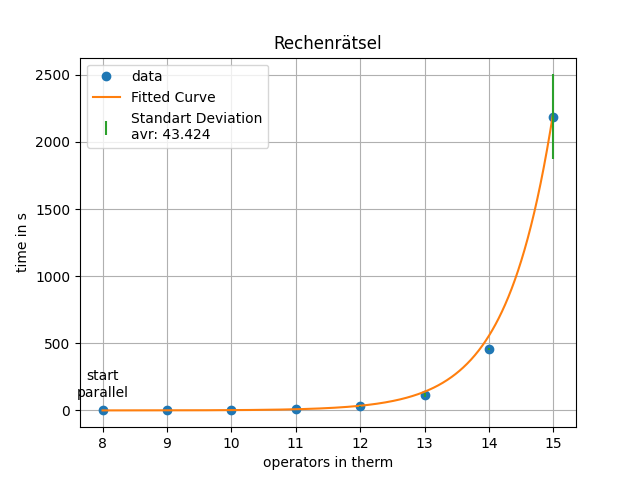
\includegraphics[width=\textwidth]{Laufzeit.png}

Wie man sieht passt diese angeglichene Funktion ziemlich gut. Der Funktionstherm wäre mit meinen Specs ca. $f(n) = 2.08e-06 \cdot 4^n$


\section{Umsetzung}
Hier wird kurz erläutert, wie die Lösungsidee im Programm tatsächlich umgesetzt wurde. Hier können auch Implementierungsdetails erwähnt werden.

\section{Beispiele}
Genügend Beispiele einbinden! Die Beispiele von der BwInf-Webseite sollten hier diskutiert werden, aber auch eigene Beispiele sind sehr gut – besonders wenn sie Spezialfälle abdecken. Aber bitte nicht 30 Seiten Programmausgabe hier einfügen!

\section{Quellcode}
Unwichtige Teile des Programms sollen hier nicht abgedruckt werden. Dieser Teil sollte nicht mehr als 2–3 Seiten umfassen, maximal 10.

\section{Erweiterung}



\end{document}
